\documentclass{tstextbook}

\begin{document}

\tsbook{Projet Tatamis}
       {Author Name}
       {Cover Designer}
       {2021-2022}
       {xxxxx}{xxx--xx--xxxx--xx--x}{0.0}
       {Publisher}
       {City}

%---------------------------------------------------------------------------
% Chapters
%---------------------------------------------------------------------------

%---------------------------------------------------------------------------
\chapter{Présentation}

\begin{summary}
  Ce premier chapitre sera l'occasion d'introduire le projet tel qu'il a été initié et de 
  détailler les outils et les méthodes utilisées lors de son développement.
\end{summary}

\section{Proposition initiale du projet}

  \subsection{Descriptif de la problématique}


    Le pavage du plan avec des rectangle est un problème classique et déjà largement documenté,
    mais je souhaite l'aborder par un aspect très concret : étant donné un nombre de tatamis, quelles sont les 
    configurations possibles.\\
    \begin{center}
        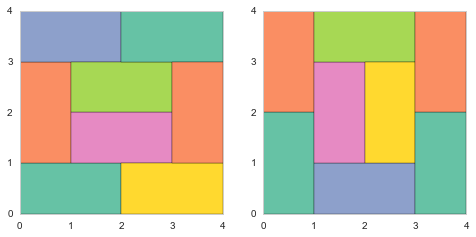
\includegraphics[width = 0.5\linewidth]{images/pavage-par-tatamis.png}
    \end{center}
    C'est un problème que rencontre notamment toute personne qui se retrouve à devoir installer un dojo.
    Il existe une contrainte de base qui est que 4 tatamis ne rejoignent jamais en un même coin. Mais ont peut
    en ajouter d'autres : possibilité de demi-tatamis (carré), répartition des couleurs, répartition de l'usure...

  \subsection{Cahier des charges}

    Utilisateur final : gestionnaire de dojo\\

    L'interface utilisateur devra comprendre un menu de paramétrage basique : nombre de tatamis,
    contraintes géométriques, contraintes d'aspect général; ainsi qu'un affichage des dispositions envisageables.\\

    L'utilisateur devra pouvoir saisir :

    \begin{itemize}
        \item le nombre et le type (entier/demis) de tatamis à disposition
        \item leurs dimensions
        \item leurs couleurs
        \item éventuellement leur état (on dispose de préférence les plus usés en périphérie)
        \item les dimensions du dojo
    \end{itemize}

    L'affichage proposera différentes disposition selon les contraintes imposées.

  \section{Membres du projet}

  
\chapter{Méthodologie}
\section{Choix de méthodologie}

La méthodologie agile nous paraît très adaptée au développement de notre programme.
En effet, la méthodologie agile:

\begin{itemize}
    \item  Est particulièrement adaptée à la résolution de problème complexes
          et incertaines ou l’on ne sait pas forcément avec précisions l’objectif
          final ou la manière d’y arriver, ce qui est notre cas
    \item Est basée sur l'itération avec la production de livrables testables
          à la fin de chaque \emph{sprint}, ce qui semble adapté pour produire nos différentes
          versions (alpha, beta…)
    \item Est basée sur une équipe multidisciplinaire qui couvre toutes les compétences
          pour produire un produit fini et qui s’auto organise, ce qui parait également
          adapté à notre contexte
\end{itemize}

La méthodologie agile, étant particulièrement adaptée aux situations d'incertitude, préconise
une planification au fur et à mesure de temps, plutôt que d’importantes et lourdes activités de 
planification en début de projet car les informations manquent pour cette planification totale en amont.

Pour nous donner un cadre, nous nous inspirons très fortement du schéma “Scrum” et du guide Scrum1, 
tout en l’adaptant à notre situation présente avec des ressources limitées et des contraintes particulières.

\section{Les événements}

\subsection{Les sprints et les phases du projet}


Les sprints sont des périodes de développement ayant un objectif précis et permettant d'arriver à une version du programme. 
Compte tenu du planning imposé par l’exercice, les sprints seront de durée variable et d'une durée légèrement supérieur à un 
mois (contrairement à ce qui est suggéré par le schéma Scrum).\\

Les sprints commencent par la session de planning et se terminent par la revue et la rétrospective (événements détaillés ci-après). Elles comprennent également des activités de 'raffinement' ou de préparation du prochain sprint,
 pour qu’un nouveau sprint puisse commencer immédiatement après la clôture du précédent sprint.\\

Quatre sprints sont programmés pour le projet aboutissant aux versions Alpha, Beta, Release Candidate et 
Production.\\

\emph{Nb: Une phase additionnelle de pré-développement aura lieu en amont pour la préparation du projet,
 mais est organisée de manière ad-hoc et ne peut être considérée comme un sprint. 
 Cette phase a pour objectif d’analyser la demande (le cahier des charges), de déterminer la méthodologie
 et gouvernance et de préparer le développement pour aboutir sur une roadmap, un plan de développement 
 global du programme qui sera bien sûr affiné au cours du temps.
}

\subsection{La session de planning du sprint}

Pour chaque sprint la session de planning permet de déterminer:

\begin{itemize}
    \item Le ‘Quoi’: quels éléments du backlog global peuvent être embarqué dans ce sprint pour créer le Sprint backlog
    \item Le ‘Comment’: comment chaque élément du Sprint backlog seront techniquement traités
    \item Le ‘Pourquoi’: quel objectif pour le sprint, sachant que chaque sprint doit délivrer un produit qui peut être limité en fonctionnalités mais qui fonctionne
\end{itemize}

Les décisions sont prises de la manière suivante:
\begin{itemize}
      \item Quoi et pourquoi :
       
      Les propositions d'éléments à ajouter et d’objectif du sprint viennent du product owner. L'équipe de développement prend ensuite la décision de manière souveraine
       et autonome en session de planification.
       \item Comment :
       
       Chaque élément du Sprint backlog est discuté techniquement pour le décomposer en plus petites tâches qui feront l’objet de tickets. 
       
       En cas de manque de compétences techniques, des tickets sont prévus pour la réalisation de recherches.
       
       Cette session couvre également les questions d’architecture du programme: choix du nombre de classes, de leurs interactions…

\end{itemize}

\subsection{"L'hebdo"}

Compte tenu de la situation particulière, un point de contact quotidien comme préconisé par le schéma Scrum n’est pas envisageable.
 Il sera remplacé par:
 \begin{itemize}
       \item Un point hebdomadaire facilité par le Scrum master pour un focus particulier sur l'échange,
        les challenges et solutions. 
       \item La revue des tâches et le statut sont quand à eux discutés à travers:
       \begin{itemize}
             \item Une communication continue sur Slack
             \item Une mise à jour en direct des avancées sur Redmine, directement sur les tâches. Redmine apportant la visibilité nécessaire à tous les membres de l'équipe pour comprendre le statut rapidement grâce à la combinaison du diagramme Gantt, d’un tableau Kanban des tâches et d’un tableau de roadmap qui suit le pourcentage de complétude du backlog du sprint

       \end{itemize}
 \end{itemize}


\subsection{La revue du sprint}

Chaque sprint se termine par une revue du produit livré à la fin du sprint. Les fonctionnalités développées sont discutées, ainsi que les challenges rencontrés.
L'équipe commence à se projeter également sur le prochain sprint et ce qu’il faut faire ensuite.

\subsection{La retrospective}
L’objectif de cette réunion est une introspection pour une amélioration continue notamment de la collaboration au sein de l'équipe, les processus et les outils.
La session est facilitée par le Scrum master et se déroule selon les principes suivants:

\begin{itemize}
      \item Discussions autour de 3 blocs successivement:
      \begin{itemize}
            \item ‘Garde’: ce que l’on considère adapté et a conserver dans le futur
            \item ‘Start’: ce que l’on souhaite commencer a faire pour améliorer la situation
            \item ‘Stop’: ce que l’on souhaite arrêter sur un constat d'échec
      \end{itemize}
      \item Étapes de chaque blocs:
      \begin{itemize}
            \item Réflexion individuelle de points/idées à ajouter pour le bloc discute
            \item Discussion de groupe pour regrouper les points mentionnés par thème
            \item Résumé des actions/idées retenues
      \end{itemize}
      \item La session se termine par la détermination du plan d'amélioration regroupant les 
      idées retenues et en ajoutant une composante de temps et responsabilité des actions
      \item Outil utilisé pour la session: Miro (outil interactif et collaboratif permettant notamment de créer et arranger facilement des ‘post it’ représentant les points/idees)
\end{itemize}

\section{Les éléments de formalisation}

\subsection{Cahier des charges global (et les Epics)}

\subsection{Le backlog global (et les User Stories)}

\subsection{Roadmap globale}

\subsection{Le backlog d’un sprint (et les Tâches)}

\section{Les rôles}

\subsection{Description des rôles}

\subsection{Assignation des rôles}

\section{L'approche de test}

 


\chapter{Choix des outils et langages}
\section{Outils de communications}

\subsection{Redmine}

Cet outil de gestion de projet a été choisi en premier lieu pour sa disponibilité immédiate (il n'y a pas eu d'installation
ou de paramétrage de serveur à réaliser) mais aussi pour sa complétude en terme d'outils. Il dispose
en effet de l'ensemble des fonctionnalités dont nous avions besoin pour ce qui est de la création, de l'ordonnancement
et du suivi des demandes. En cela il est tout à fait adapté à la méthodologie choisie.\\

Nous avons pu le paramétrer un peu plus finement de façon à ce que les caractéristiques et l'évolution des demandes
correspondent à la terminologie employée pour détailler notre projet : type de tracker, statut des demandes, champs personnalisés\dots


\subsection{Slack}

Slack a été choisi comme outil de communication entre les membres de l'équipe afin d'établir des canaux de discussion différenciés. 
Cela permet à l'équipe des échanges plus ciblés et donc plus efficaces, ainsi qu'une vision plus ordonnée de l'historique des communications.

\subsection{Github}

La plateforme Github a été choisie pour héberger et gérer l'ensemble des éléments du projet, à savoir
le code de l'application ainsi que le rapport.

Le dépot est consultable à l'adresse : \url{https://github.com/bubobou/tatamis}

\section{Développement}

\subsection{Langage}

De part sa facilité d'assimilation et les nombreuses bibliothèques disponibles, le choix du langage de programmation
s'est porté sur Python dans sa version 3.9.

\subsection{Bibliothèques}

Différentes bibliothèques nous ont parues d'emblée utiles pour aborder ce projet. Tout d'abord
une recherche documentaire nous a menée vers la bibliothèque \textsf{facile} permettant de traiter
de la programmation par contrainte. Même s'il ne sera pas forcément retenue dans la version finale, 
sa disponibilité nous permet d'aborder plus sereinement notre problématique.\\

Par ailleurs dans la finalité d'une application avec interface graphique, potentiellement portée sur terminal mobile,
 nous avons envisagé l'utilisation de bibliothèques et d'utilitaires tels que :

 \begin{itemize}
     \item \textsf{PyQt}
     \item \textsf{Kivy}
     \item \textsf{python for android}
 \end{itemize}

\chapter{Cahier des charges}
\section{Démarche}

La problématique initiale telle qu'elle a été énoncée est la suivante : \emph{étant donné un nombre de tatamis, quelles sont les 
configurations possibles ?}\\


Nous allons ici détaillé plus précisément le cahier des charges de l'application afin d'en déduire
les users stories et leurs tâches afférentes, et ainsi d'établir la roadmap de notre projet. Le cahier des charges est formulé 
du point de vue de l'utilisateur final, en les rédigeant sous la forme : \emph{en tant que} \dots ,\emph{je souhaite} \dots ,\emph{afin de } \dots.\\


Par ailleurs afin de prioriser les demandes, nous les classerons en deux catégories :

\begin{itemize}
    \item essentielles (must have)
    \item optionnelles (nice to have)
\end{itemize}

\section{Fonctionnalités essentielles}

%\item \emph{En tant que } gestionnaire de dojo,\emph{ je souhaite} ... \emph{ afin de }...

\begin{itemize}
    \item \emph{En tant que} gestionnaire de dojo, \emph{ je souhaite} savoir s'il existe une solution utilisant l'ensemble de mes tatamis,
    \emph{afin de } savoir si je pourrai tous les utiliser.
    \item \emph{En tant que} gestionnaire de dojo,\emph{ je souhaite} connaître le nombre de tatamis utilisables \emph{ afin de }
     n'en déployer que le nombre nécessaire.
    \item \emph{En tant que} gestionnaire de dojo  ,\emph{je souhaite} visualiser l'ensemble des dispositions possibles, modulo une rotation ou une symétrie
    \emph{afin de } ne voir sur l'écran que les solutions réellement différentes.
    \item \emph{En tant que} gestionnaire de dojo, \emph{ je souhaite} pouvoir renseigner le nombre de tatamis dont je dispose,
    \emph{afin de } d'obtenir une solution adaptée à mon matériel.
    \item \emph{En tant que} gestionnaire de dojo,\emph{ je souhaite} pouvoir renseigner les dimensions de mon dojo \emph{ afin d'}
     obtenir une solution adaptée à l'espace dont je dispose.    
    \item \emph{En tant que} gestionnaire de dojo,\emph{ je souhaite} voir afficher les dimensions (longueur, largeur, surface) des dispositions 
    proposées  \emph{ afin d' }exploiter aux mieux l'espace disponible à l'intérieur et à l'extérieur du tatamis.
\end{itemize}

\chapter{Backlog global}
\input{sections/backlog-global.tex}

\chapter{Roadmap globale}
\section{Roadmap au 08/01/2022}

\subsection{Éléments}

\noindent%
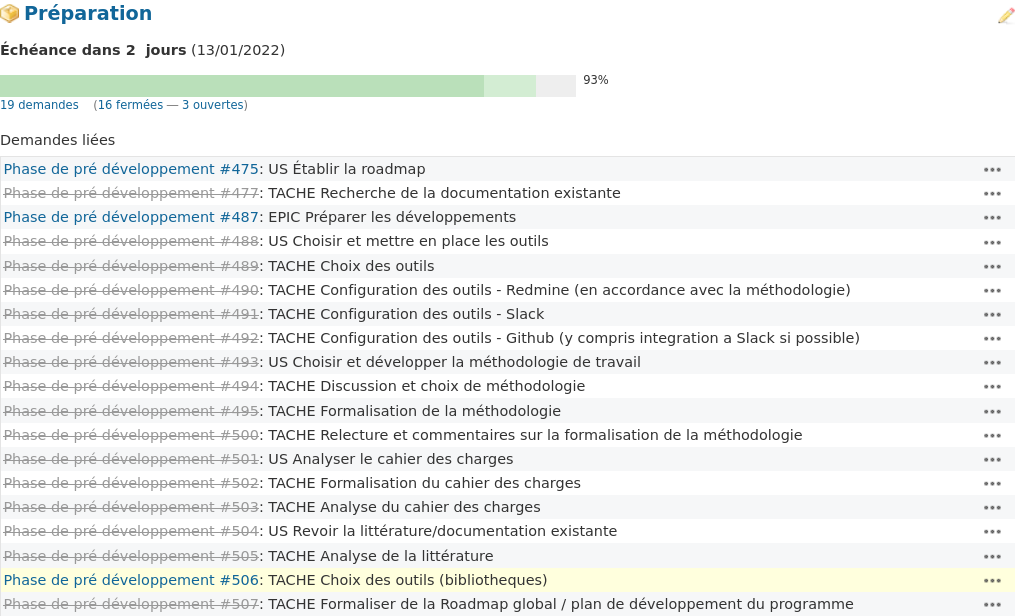
\includegraphics[scale=0.5]{images/roadmap_prepa.png}

\noindent%
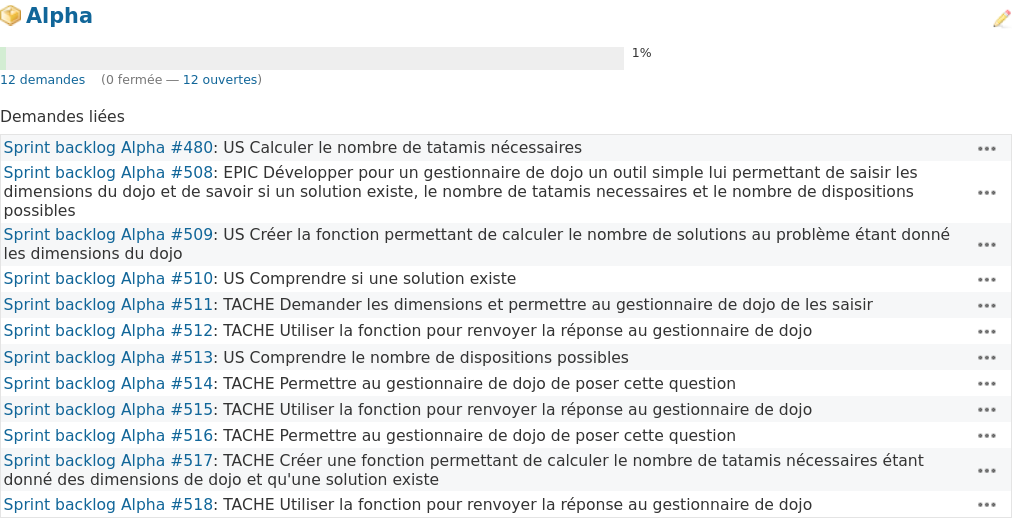
\includegraphics[scale=0.5]{images/roadmap_alpha.png}\\
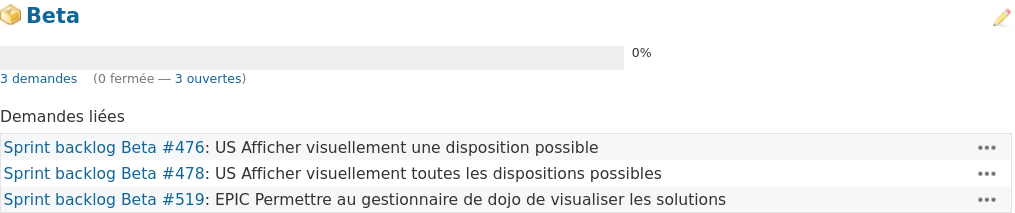
\includegraphics[scale=0.5]{images/roadmap_beta.png}\\
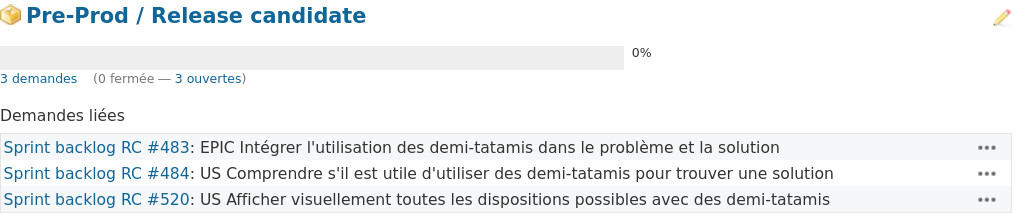
\includegraphics[scale=0.5]{images/roadmap_RC.png}\\
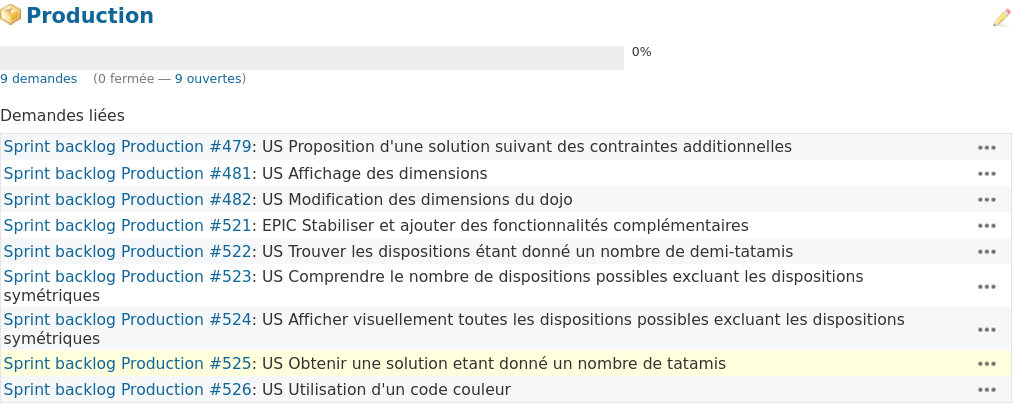
\includegraphics[scale=0.5]{images/roadmap_prod.png}

\subsection{Gantt}

\noindent%
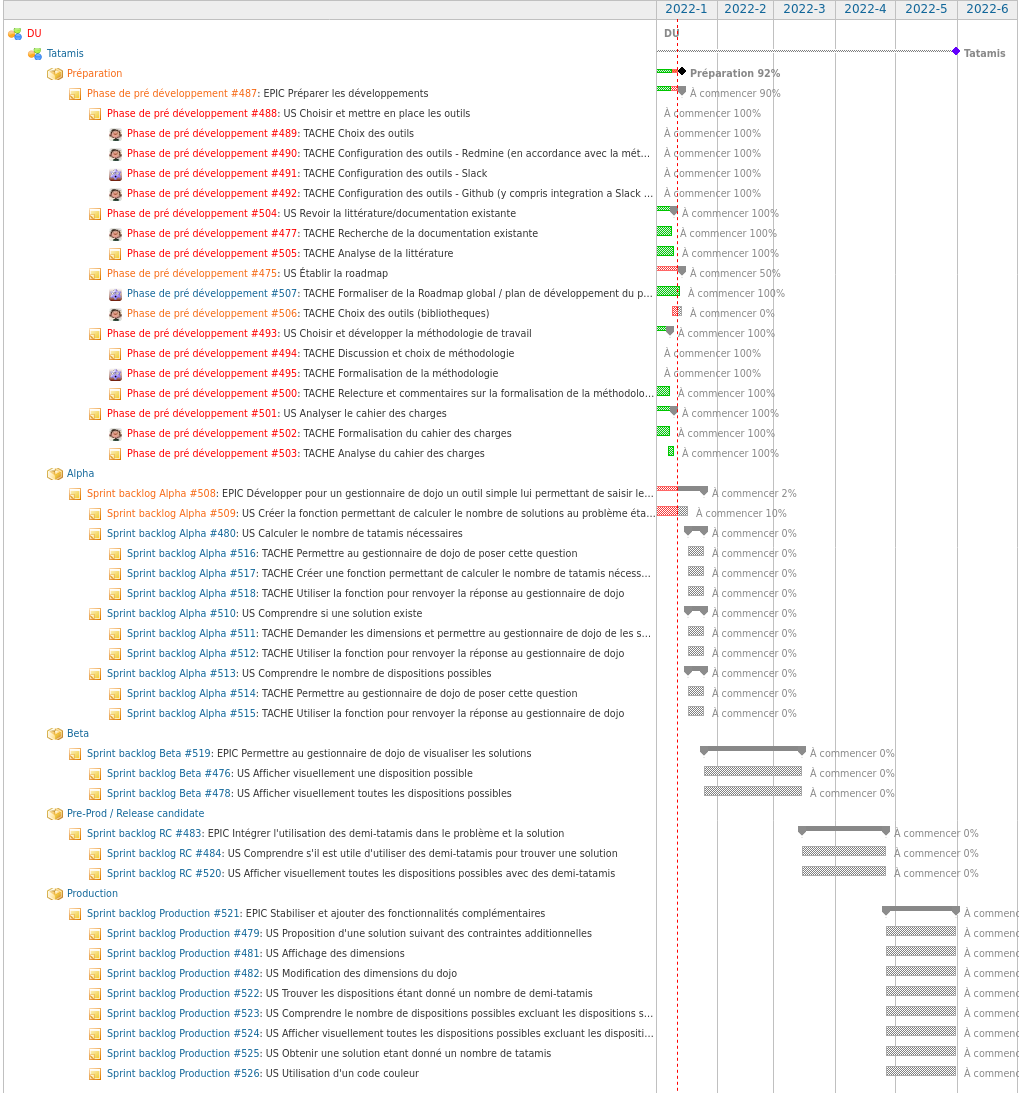
\includegraphics[scale=0.55]{images/Gantt0801.png}


\chapter{Backlog de chaque sprint}
\input{sections/backlog-sprint.tex}

\chapter{Explication de l'algorithme}
\input{sections/explication-algorithme.tex}

\chapter{Choix de programmation}
\input{sections/choix-programmation.tex}

\chapter{Tests}
\input{sections/tests.tex}

\chapter{Gestion des versions concurrentes}

\end{document}